\begin{flushleft}

%\addcontentsline{toc}{chapter}{Development Process}
\chapter{Design}
\label{Design}

This section will describe the design as of the date of the project outline description. \\
This is the design which will be followed and tried to implement, however this is more of a guideline rather than exact plan since at this moment it is uncertain what the  API and simulator are able to do and what is possible to implement inside the given time.\\

\section{Environment Design}
The final environment for this project will consist of one large room with obstacles placed in it. \\
The program will be tested on a number of different sized rooms with different amount and sized obstacles in it.


\begin{figure}[h]
\centering
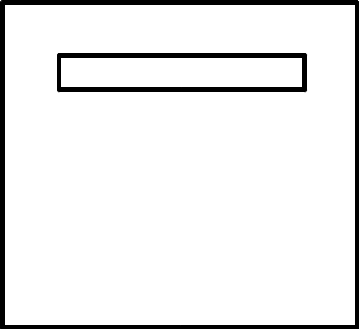
\includegraphics[width=0.5\textwidth]{../../figures/environment_example2.png} 
\caption{Environment Design}
\label{Figure 2}
\end{figure}

\section{Mapping and Swarm Size}
For mapping I will use a occupancy grid, and the occupancy will be acquired by the E-Puck's laser sensors. 
I will yet have to decide on a resolution, for the grid.\\
I will use a swarm of 5 E-Puck robots, of which 1 will remain stationary and only function as the "Uplink point" to which all robot send the acquired data. 
The stationary robot will also be used as reference point for the localisation method.

\section{Deployment}
It is at this moment still undecided which deployment strategy will be implemented. \\
There are 2 deployment strategies which are based on the background research which has been done.\\[3ex]

\subsection{Considered Deployment algorithms}

One which is based on a random walk though the environment which will turn to a random heading when an obstacle has been reached. \\
This approach could be combined with a wall following algorithm which would trigger a random walk when the same position is reached again. This would allow for the complete traverse of a obstacle/wall. This would require a good localisation solution as without it the robot will be stuck inside an eternal loop.\\[3ex]

The other deployment strategy would implement a more controlled movement pattern. This pattern would move the robots inside a rectangular pattern which would implement a function to move around obstacles on the way before moving back into the original pattern. 
While this reason is more controlled I am not sure which one will turn out to be more effective, that it why I will implement both inside a testing phase and will then decide which of them I will use.

\begin{figure}[h]
\centering
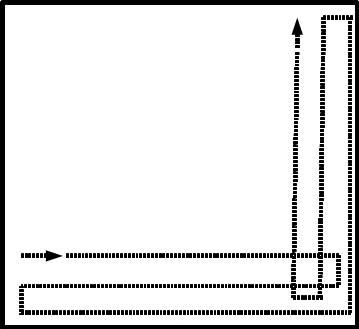
\includegraphics[width=0.5\textwidth]{../../figures/movement_pattern.png} 
\caption{Controlled movement Pattern}
\label{Figure 3}
\end{figure}

\subsection{Adopted design}
It was decided to adopt and implement the more controlled movement pattern which can be seen in figure \ref{Figure 3}.\\
The reason for this being that the developer believes a random walking approach, because of its random behaviour, would be sub-optimal in a more complex environment whereas the controlled movement pattern would perform better. This is assumed as for future implementation more complex environments and possibly multi-robot usage is planned, however more about this can be found in chapter \ref{Future_plans}  on page \pageref{Future_plans}.

\end{flushleft}
